\documentclass[xcolor=dvipsnames,handout]{beamer}

% font setup
\usepackage{libertine}
\renewcommand*\familydefault{\sfdefault}    % Linux Libertine = default sans serif
\usepackage{inconsolata}                    % Inconsolata = monospaced
\usepackage[utf8]{inputenc}
\usepackage[T1]{fontenc}
\usepackage{tikz}
\usetikzlibrary{positioning}

\usepackage{algorithm}
\usepackage{algpseudocode}
\makeatletter
\renewcommand{\ALG@name}{Algoritm}
\makeatother
\algrenewcommand\algorithmicprocedure{\textbf{procedură}}
\algrenewcommand\algorithmicend{\textbf{final}}

% Graphics and other packages
\usepackage[romanian]{babel}
\usepackage{graphicx}
\addto\captionsromanian{\renewcommand{\figurename}{Ilustrație}}
\usepackage{caption}
\usepackage{subcaption}
\usepackage[style=german]{csquotes}

% Custom macros
\newcommand{\bloc}[3]{\begin{bl}<#1->{{\large\color{Gray}{\hrulefill}}\\ \color{bleumarin}{\large \emph{#2}}}\\ \vspace*{-2mm}{\color{Gray}{\hrulefill}}\\ #3 \end{bl}} 
\newcommand{\fr}[1]{\frame{#1}}
\newcommand{\ft}[1]{\frametitle{\color{bleumarin}{\hfill #1 \hfill}}}
\newcommand{\lin}[3]{\uncover<#1->{\alert<#1>{#2}}{\vspace*{#3 ex}}}
\newcommand{\ite}[2]{\uncover<#1->{\alert<#1>{\item #2}}}
\newcommand{\vs}[1]{\vspace*{#1 ex}}
\definecolor{bleumarin}{RGB}{30,30,150} 
\definecolor{firebrick}{RGB}{178,34,34}

% Theme setup
\useoutertheme{shadow} 
\usetheme{CambridgeUS} 
\usecolortheme[named=bleumarin]{structure} 
\useoutertheme[compress]{smoothbars}

% Theme finetuning
\setbeamertemplate{items}[ball]
\setbeamertemplate{blocks}[rounded][shadow=true]
\setbeamertemplate{navigation symbols}{}
\setbeamertemplate{headline}{}  


%%%%%%%%%%%%%%%%%%%%%%%%%%%%%%%%%%%%%%%%%%%%%%%%%%%%%%%%%%%%%%%%%%%%%% 
% TITLE PAGE
\title{Definiții accesibile \\ (\emph{Reaching definitions})}
\author{Adrian Manea}
\institute{510, SLA}

\date{}

\begin{document}

\maketitle

% SLIDES START HERE
%%%%%%%%%%%%%%%%%%%%%%%%%%%%%%%%%%%%%%%%%%%%%%%%%%%%%%%%%%%%%%%%%%%%%% 
\fr{
  \ft{Teorie}

  \lin{1}{Definiții accesibile = reaching definitions}{2}

  \lin{2}{= Definiții care se propagă pînă la punctul curent al analizei.}{2}

  \lin{3}{O definiție poate fi \emph{generată} (\texttt{gen}) sau
    \emph{distrusă} (suprascrisă, \texttt{kill}).}{2}

  \lin{4}{Analiza folosește \emph{funcții de transfer} în ecuații \texttt{gen-kill}:
    \[
      f_d(x) = \texttt{gen(d)} \cup (x - \texttt{kill(d)}).
    \]
  }{4}
}

\fr{
  \ft{Exemplu (Aho et al.)}

  \begin{figure}[!htbp]
    \centering
    \usetikzlibrary{positioning}
    \usetikzlibrary{shapes.geometric}
    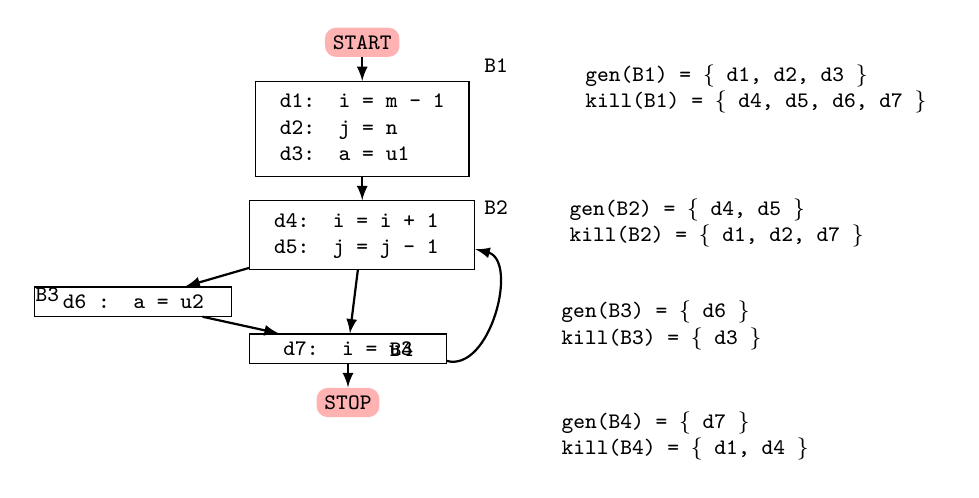
\begin{tikzpicture}[node distance=0.3cm,
      startstop/.style={rectangle,rounded corners,text centered,fill=red!30},
      process/.style={rectangle, minimum width=2.5cm, draw=black},
      arr/.style={thick,-latex}
      ]
      \footnotesize
      \node (in) [startstop] {\texttt{START}};
      \node (b1) [process,below=of in] 
      {\begin{tabular}{l} \texttt{d1: i = m - 1} \\ \texttt{d2: j = n} \\ \texttt{d3: a = u1} \end{tabular}};
      \draw[arr] (in) -- (b1);
      \node at (1.7,-0.3) {\texttt{B1}};
      \node at (5, -0.6) {\begin{tabular}{l} \texttt{gen(B1) = \{ d1, d2, d3 \}} \\ \texttt{kill(B1) = \{ d4, d5, d6, d7 \}} \end{tabular}};
      \node (b2) [process,below=of b1]
      {\begin{tabular}{l} \texttt{d4: i = i + 1} \\ \texttt{d5: j = j - 1 } \end{tabular}};
      \draw[arr] (b1) -- (b2);
      \node at (1.7,-2.1) {\texttt{B2}};
      \node at (4.5, -2.3) {\begin{tabular}{l} \texttt{gen(B2) = \{ d4, d5 \}} \\ \texttt{kill(B2) = \{ d1, d2, d7 \}}\end{tabular}};
      \node (b3) [process, below left=of b2] {\texttt{d6 : a = u2}};
      \draw[arr] (b2) -- (b3);
      \node at (-4,-3.2) {\texttt{B3}};
      \node at (3.8, -3.6) {\begin{tabular}{l} \texttt{gen(B3) = \{ d6 \}} \\ \texttt{kill(B3) = \{ d3 \}} \end{tabular}};
      \node (b4) [process, below right=of b3] {\texttt{d7: i = u3}};
      \draw[arr] (b3) -- (b4);
      \draw[arr] (b2) -- (b4);
      \draw[arr,bend right=90] (b4) to (b2);
      \node at (0.5,-3.9) {\texttt{B4}};
      \node at (4.1, -5) {\begin{tabular}{l} \texttt{gen(B4) = \{ d7 \}} \\ \texttt{kill(B4) = \{ d1, d4 \}} \end{tabular}};
      \node (out) [startstop, below=of b4] {\texttt{STOP}};
      \draw [arr] (b4) -- (out);
    \end{tikzpicture}
    \caption{Exemplu pentru definiții accesibile}
    \label{fig:rdef-ex1}
  \end{figure}
}

\fr{
  \ft{Algoritm iterativ}

  \begin{algorithm}[H] % force rendering, not well supported by beamer
    \caption{Algoritm iterativ pentru definiții accesibile}
    \begin{algorithmic}[1]
      \Procedure{RDEF}{B}
      \State $ \texttt{OUT[START]} = \emptyset $
      \For{($\texttt{B} \neq \texttt{START}$)}
      \State $ \texttt{OUT[B]} = \emptyset $
      \EndFor
      \While{(\texttt{OUT} se schimbă)}
      \For{($\texttt{B} \neq \texttt{START}$)}
      \State $ \texttt{IN[B]} = \bigcup_{\texttt{P} \downarrow \texttt{B}} \texttt{OUT[P]} $
      \State $ \texttt{OUT[B]} = \texttt{gen(B)} \cup (\texttt{IN[B]} - \texttt{kill(B)}) $
      \EndFor
      \EndWhile
      \EndProcedure
    \end{algorithmic}
    \label{alg:rdef}
  \end{algorithm}
}

\fr{
  \ft{Exemplu (Aho et al.)}

  \begin{figure}[!htbp]
    \centering
    \usetikzlibrary{shapes.geometric}
    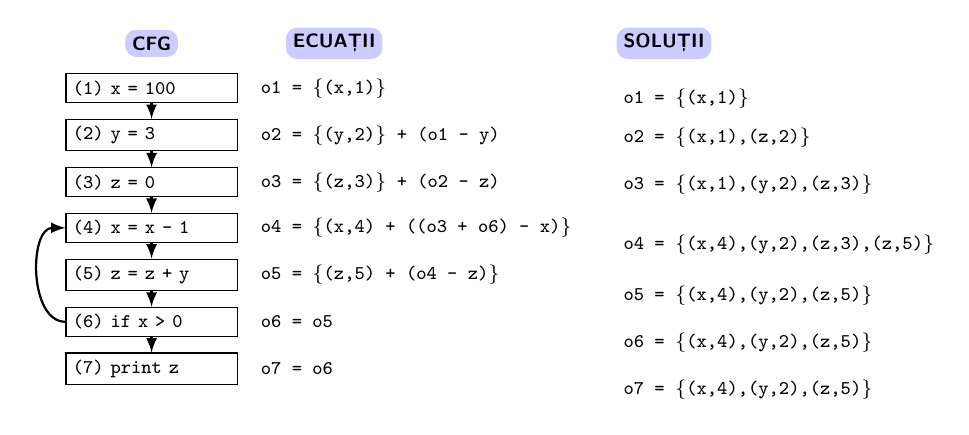
\begin{tikzpicture}[node distance=0.2cm,
      startstop/.style={rectangle,rounded corners,text centered,fill=blue!20},
      process/.style={rectangle, text width=2cm, draw=black},
      arr/.style={thick,-latex}
      ]
      \scriptsize
      \node (cfg) [startstop] at (0,0)              { \textbf{CFG} };
      \node (eq)  [startstop,right=of cfg] at (1.5,0) { \textbf{ECUAȚII} };
      \node (sol) [startstop, right=of eq] at (5.7,0) { \textbf{SOLUȚII} };
      \node (1) [process, below=of cfg] {\texttt{(1) x = 100}};
      \node (2) [process, below=of 1] {\texttt{(2) y = 3}};
      \node (3) [process, below=of 2] {\texttt{(3) z = 0}};
      \node (4) [process, below=of 3] {\texttt{(4) x = x - 1}};
      \node (5) [process, below=of 4] {\texttt{(5) z = z + y}};
      \node (6) [process, below=of 5] {\texttt{(6) if x > 0}};
      \node (7) [process, below=of 6] {\texttt{(7) print z}};
      \draw[arr] (1) -- (2) ;
      \draw[arr] (2) -- (3) ;
      \draw[arr] (3) -- (4) ;
      \draw[arr] (4) -- (5) ;
      \draw[arr] (5) -- (6) ;
      \draw[arr] (6) -- (7);
      \draw[arr,bend left=90] (6) to (4);
      \node (e1) [right=of 1] {\texttt{o1 = \{(x,1)\}}};
      \node (e2) [right=of 2] {\texttt{o2 = \{(y,2)\} + (o1 - y)}};
      \node (e3) [right=of 3] {\texttt{o3 = \{(z,3)\} + (o2 - z)}};
      \node (e4) [right=of 4] {\texttt{o4 = \{(x,4) + ((o3 + o6) - x)\}}};
      \node (e5) [right=of 5] {\texttt{o5 = \{(z,5) + (o4 - z)\}}};
      \node (e6) [right=of 6] {\texttt{o6 = o5}};
      \node (e7) [right=of 7] {\texttt{o7 = o6}};
      \node (s1) [right=of e1] at (5.7,-0.7) {\texttt{o1 = \{(x,1)\}}};
      \node (s2) [right=of e2] at (5.7,-1.2) {\texttt{o2 = \{(x,1),(z,2)\}}};
      \node (s3) [right=of e3] at (5.7,-1.8) {\texttt{o3 = \{(x,1),(y,2),(z,3)\}}};
      \node (s4) [right=of e4] at (5.7,-2.55) {\texttt{o4 = \{(x,4),(y,2),(z,3),(z,5)\}}};
      \node (s5) [right=of e5] at (5.7,-3.2) {\texttt{o5 = \{(x,4),(y,2),(z,5)\}}};
      \node (s6) [right=of e6] at (5.7,-3.8) {\texttt{o6 = \{(x,4),(y,2),(z,5)\}}};
      \node (s7) [right=of e6] at (5.7,-4.4) {\texttt{o7 = \{(x,4),(y,2),(z,5)\}}};
    \end{tikzpicture}
    \caption{Exemplu pentru definiții accesibile}
    \label{fig:def-epfl}
  \end{figure}
}

\fr{
  \ft{Variabile neinițializate}

  \begin{figure}[!htbp]
    \centering
    \usetikzlibrary{shapes.geometric}
    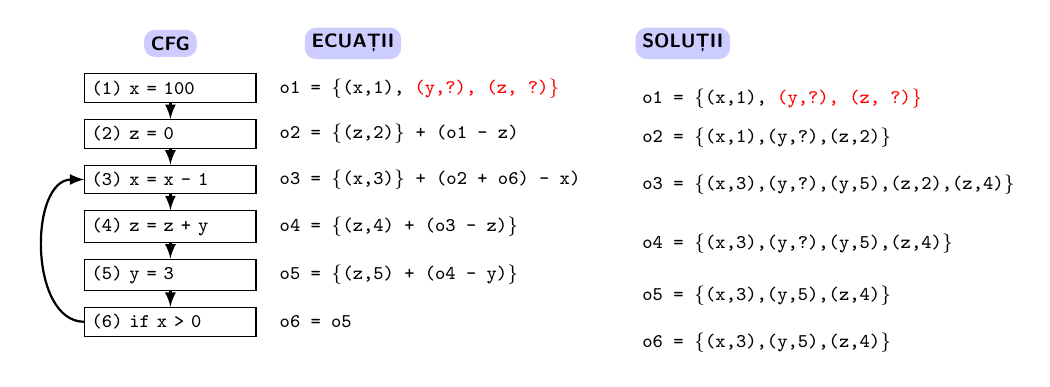
\begin{tikzpicture}[node distance=0.2cm,
      startstop/.style={rectangle,rounded corners,text centered,fill=blue!20},
      process/.style={rectangle, text width=2cm, draw=black},
      arr/.style={thick,-latex}
      ]
      \scriptsize
      \node (cfg) [startstop] at (0,0)              { \textbf{CFG} };
      \node (eq)  [startstop,right=of cfg] at (1.5,0) { \textbf{ECUAȚII} };
      \node (sol) [startstop, right=of eq] at (5.7,0) { \textbf{SOLUȚII} };
      \node (1) [process, below=of cfg] {\texttt{(1) x = 100}};
      \node (2) [process, below=of 1] {\texttt{(2) z = 0}};
      \node (3) [process, below=of 2] {\texttt{(3) x = x - 1}};
      \node (4) [process, below=of 3] {\texttt{(4) z = z + y}};
      \node (5) [process, below=of 4] {\texttt{(5) y = 3}};
      \node (6) [process, below=of 5] {\texttt{(6) if x > 0}};
      \draw[arr] (1) -- (2) ;
      \draw[arr] (2) -- (3) ;
      \draw[arr] (3) -- (4) ;
      \draw[arr] (4) -- (5) ;
      \draw[arr] (5) -- (6) ;
      \draw[arr,bend left=90] (6) to (3);
      \node (e1) [right=of 1] {\texttt{o1 = \{(x,1), {\color{red} \textbf{(y,?), (z, ?)}\}}}};
      \node (e2) [right=of 2] {\texttt{o2 = \{(z,2)\} + (o1 - z)}};
      \node (e3) [right=of 3] {\texttt{o3 = \{(x,3)\} + (o2 + o6) - x)}};
      \node (e4) [right=of 4] {\texttt{o4 = \{(z,4) + (o3 - z)\}}};
      \node (e5) [right=of 5] {\texttt{o5 = \{(z,5) + (o4 - y)\}}};
      \node (e6) [right=of 6] {\texttt{o6 = o5}};
      \node (s1) [right=of e1] at (5.7,-0.7) {\texttt{o1 = \{(x,1), {\color{red} \textbf{(y,?), (z, ?)}\}}}};
      \node (s2) [right=of e2] at (5.7,-1.2) {\texttt{o2 = \{(x,1),(y,?),(z,2)\}}};
      \node (s3) [right=of e3] at (5.7,-1.8) {\texttt{o3 = \{(x,3),(y,?),(y,5),(z,2),(z,4)\}}};
      \node (s4) [right=of e4] at (5.7,-2.55) {\texttt{o4 = \{(x,3),(y,?),(y,5),(z,4)\}}};
      \node (s5) [right=of e5] at (5.7,-3.2) {\texttt{o5 = \{(x,3),(y,5),(z,4)\}}};
      \node (s6) [right=of e6] at (5.7,-3.8) {\texttt{o6 = \{(x,3),(y,5),(z,4)\}}};
    \end{tikzpicture}
    \caption{Exemplu pentru \texttt{y} neinițializată}
  \end{figure}

}

\fr{
  \ft{Utilizări}

  \lin{1}{Optimizare: identificarea constantelor propagate;}{4}

  \lin{2}{Identificarea variabilelor neinițializate;}{4}

  \lin{3}{Componentă esențială a analizei fluxului de date.}{4}
}

%%%%%%%%%%%%%%%%%%%%%%%%%%%%%%%%%%%%%%%%%%%%%%%%%%%%%%%%%%%%%%%%%%%%%% 

% Bibliography
\fr{
  \ft{Bibliografie}
  \bibliography{def.bib}
  \bibliographystyle{apalike}
  \nocite{*}
}
\end{document}

